%\section{Preliminary Study}

%In order to understand the insightful information of musical head movement,
Next, we conducted a preliminary experiment to investigate whether head-movement patterns can be potentially used to authenticate users. In this experiment, we collected head-movement accelerometer data from 28 subjects, wherein each subject was asked to perform a simple nodding movement following a short audio track (referred to as \emph{music cue} in the rest of the paper).   For this purpose, we examined %two simple features: (1) wave amplitude, the difference between the bottom of a wave and the peak of the following wave, which indicates how hard a person nods; %(2) mean wave width, the mean interval between two consecutive wave bottoms or peaks, which indicates the length of a nodding motion;
%and (2)
a simple aspect of the head-movement pattern, response time, which is the time interval between a music beat and the corresponding nodding motion, as shown in Figure~\ref{fig:waveform}. The response time indicates how quickly a person responds to music beats.
% we extract several characteristics from the original accelerometer data:
%\begin{itemize}
%\item{\em Wave amplitude},which is the difference of a wave bottom and its next wave peak. It measures the acceleration when the user performs the head-movement, in other words, wave amplitude describes “how hard” the user nod his head. Due to accelerometer data usually contains high frequency noise, and we are more interested in the main signal where user nod his head, a 5-Hz-cutoff low-pass filter is applied before we extract all the characteristic in the signal.
%\item{\em Wave widh}, which is the time interval between two bottoms or two peaks. It describes the time to complete one nodding movement. The user is stimulated by a music cue, wave width is effected by the time interval between beats.
%\item{\em Series of response time (SRT)},which is the series of time interval between the music beat and corresponding movement.  Studies in ~\cite{westeyn2004recognizing} and ~\cite{wobbrock2009tapsongs} show SRT could be used to differentiate the users. It is important to note that user is not necessary perform after the music beat. The evidence in music psychology ~\cite{clarke1999rhythm,fraisse1982rhythm} demonstrate that  humans have capability to perceive and perform rhythmm, hence user can perform the moving before he hears the beat.
%response time in our measurement can be either negative or positive. However, finding the associated movement of a beat is a non-trivial process, hence we develop the following algorithm to achieve this goal and form a SRT. First, accelerometer data needs to be synchronized with the music cue in midi format. Since midi file is a time series of instrument commands,  no additional signal processing is required to detect the beat in the music as we can take each command as a beat if the music is simple enough. Second, we locate two neighboring peaks where a beat resides in between, and compute the time intervals from the beat to both peaks. Finally, we choose the one with a smaller absolute value as the response time. Note that we only use data from two axis, since nodding rarely generates meaningful data on the other one. In some cases,  user is not necessary nodding for every beat,  thus we use the 90 percentile of the response time sample to interpolate  when the detected response time is beyond this value.
%\end{itemize}

\begin{figure}[t]
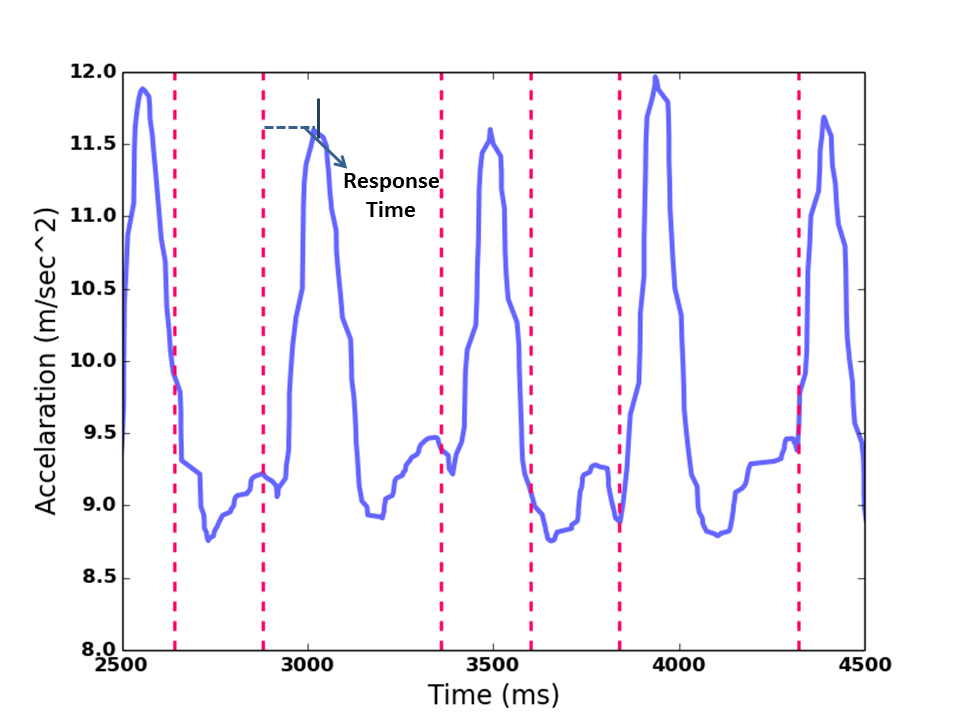
\includegraphics[width=.75\columnwidth]{figure/waveform_1.png}
\centering
\caption{\label{fig:waveform}The response time of a head motion is the interval between the motion and the music beat to which the motion responds. From a sequence of head motions, we can obtain the response time sequence.}
\end{figure}

%\begin{figure}
%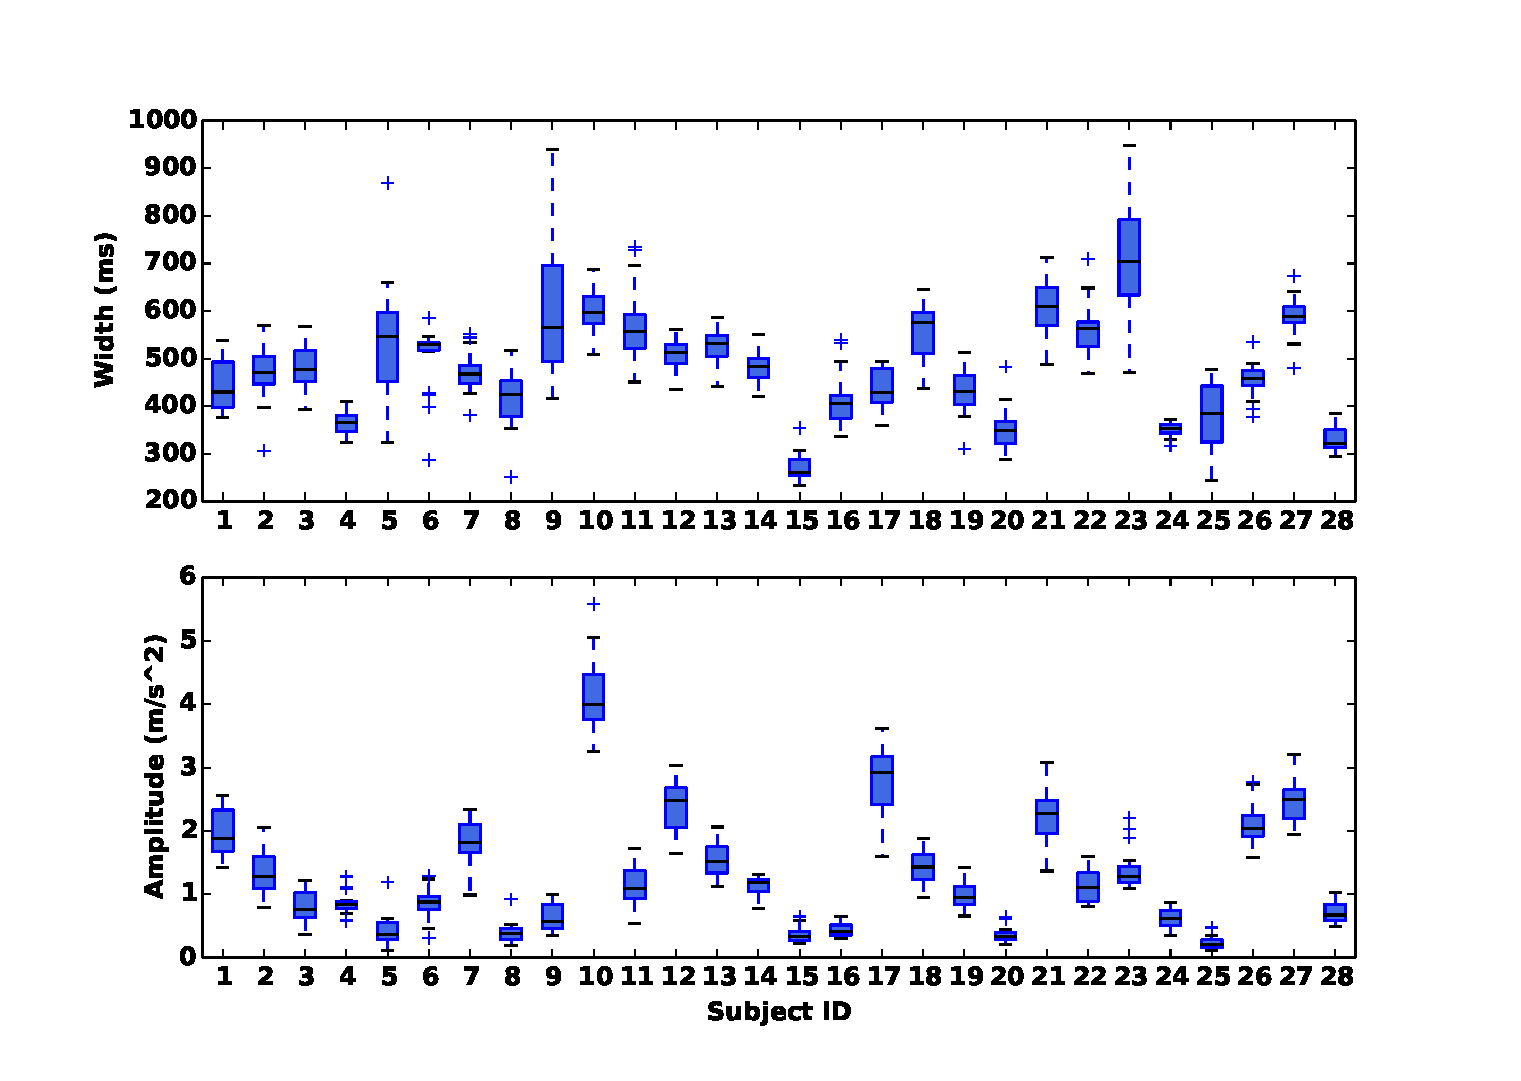
\includegraphics[width=\columnwidth]{figure/width_amp_box.eps}
%\centering
%\caption{\label{fig:width_amp} Wave Amplitude Boxplot **YZ: please re-consider the features** \textbf{ALL FIGURES SHOULD TELL WHAT IS THE TAKE-AWAY. MAKE THE PAPER GLANCEABLE, INCLUDE A PARAGRAPH FOR ALL FIGURES}}
%\end{figure}

\begin{figure*}[t]
\begin{center}
\begin{tabular}{ccc}
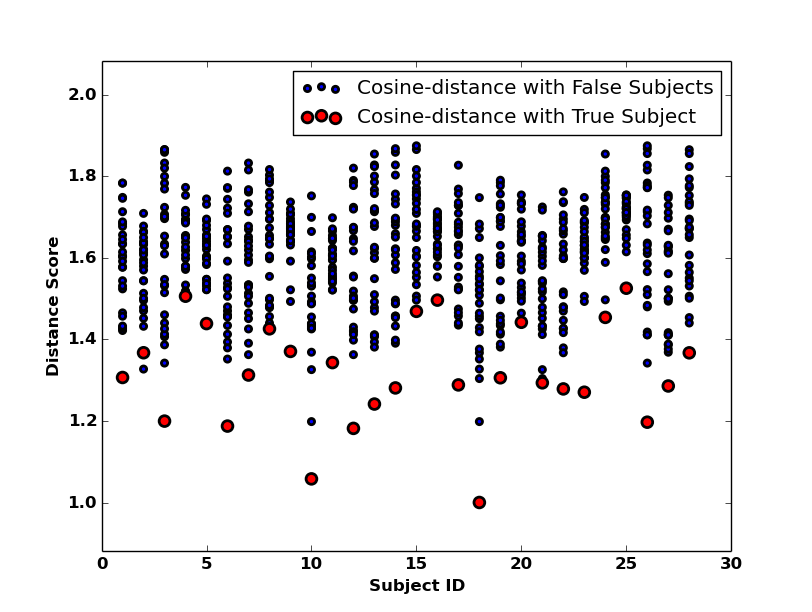
\includegraphics [width=.31\linewidth]{figure/resp_time_cos.png}&
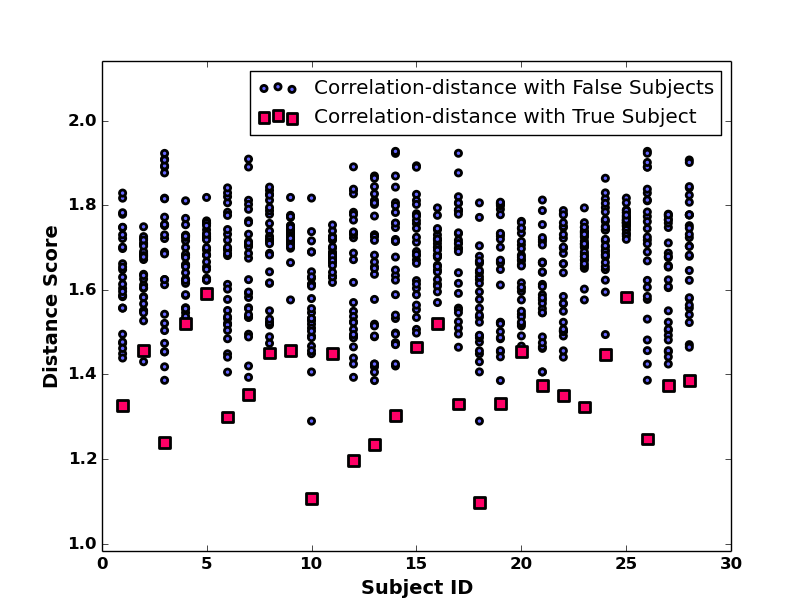
\includegraphics [width=.31\linewidth]{figure/resp_time_cor.png}&
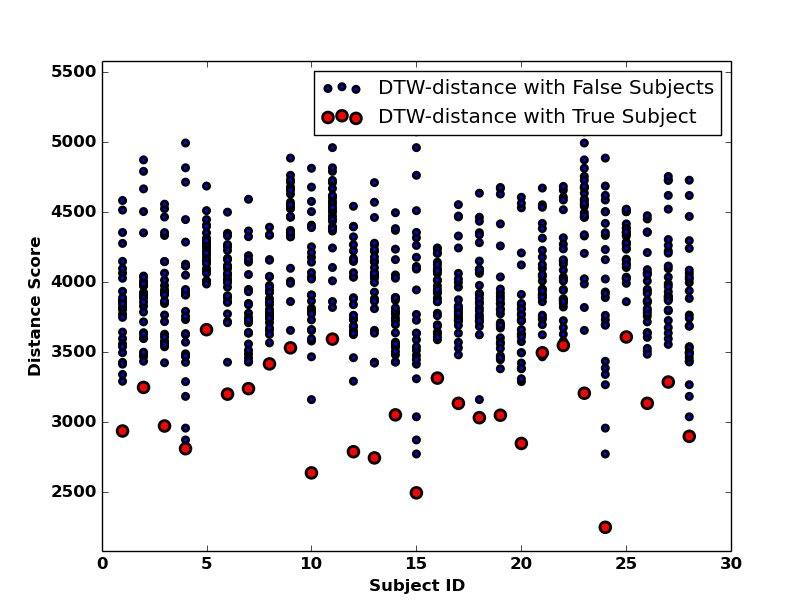
\includegraphics [width=.31\linewidth]{figure/resp_time_dtw.png}\\
(a) Cosine Distance & (b) Correlation & (c) DTW \\
\end{tabular}
\end{center}
\caption{\label{fig:distance} (a) Cosine, (b) Correlation and (c) DTW distances are computed over 20 response time time series for each subject, with 28 subjects in total. For each subject's column, a red square represents the average distance among that subject's own response times, while a blue dot represents the average distance to other subjects' response times. The results show that red distances are always lower than blue ones, suggesting that different subjects' head-movement patterns are distinguishable.}
\vspace{-2pt}
\end{figure*}


%Figure~\ref{fig:width_amp} shows each subject's wave amplitude box plot (we collected 20 nodding samples for each subject in the experiment). We observe that each subject's wave amplitude distribution ***

In this experiment, we collected 20 samples from each subject, hence 20 response time time series for each subject. Then we calculated the average distance scores between these response times, both for the same subject and across subjects. We considered three types of distance metrics: cosine distance (COS), correlation distance (COR), and dynamic time warping (DTW) distance~\cite{dtw}, and the readers can find the detailed description of these three metrics in Section~\ref{subsec:distance}. We plot these three types of distance values in Figures~\ref{fig:distance} (a)-(c), respectively. In each plot, we include distance values for all 28 subjects -- for each subject, we plot average distance scores between her and each of the other 27 subjects (referred to as distances with false subjects, shown in blue dots), as well as average distance scores among her own response times (referred to as distances with true subjects, shown in red squares). All three figures clearly demonstrate that the average distance score between a subject's samples is much lower than that among different subjects' samples, which further suggests that a subject exhibits repeatable and unique head nodding characteristics.


These observations suggest that even with simple nodding movements, the accelerometer data collected by Google Glass have the potential to be used for accurate and robust authentication. Motivated by this observation, we next devise the \systemname~authentication system.
%To better understand the SRT for different users,  we apply various similarity scores to provide an intuitive and quantitative description of their difference. In Figure~\ref{fig:distance}, the average Cosine Distance (COS) and Correlation (COR) can help most of the subject to differentiate himself with the other subjects, but for some subjects's true subject score (red dot) are closed to their false subject score (blue dot). For subject 2, red dot even exceeds the blue dot.The output of Dynamic Time Warping (DTW)~\cite{cite dtw} can be used as another distance metric.In Figure~\ref{fig:resp_time_dtw},  it shows that all average self-comparing similarity scores are lower than that when they are compared with false users. In real world, the SRT detection algorithm may not be practical if we also consider more complex head-movement other than simple nodding for each beat. The observation above indicates the possibility to further derive a system which can differentiate the true user and the false users based on the fusion of these characteristics.
